\chapter{Abstract}\label{ch:abstract}
\section{Introduction}\label{sec:introduction}
For decades, especially with the development of big data, the amount of information moving over the internet that companies must control has increased dramatically, and this growth is estimated at 78 \% per year.

All the distribution, storage and processing of information has been decentralized and is no longer carried out in the offices themselves, instead it is done in specialized rooms, called \textit{Data Processing Centres} or \textit{DPC}.

These rooms are equipped with the necessary IT equipment to perform all the above tasks and to ensure optimal working conditions and facilitate maintenance. In addition, they have various control and security systems that make it possible to detect any type of incident that could slow down processes or cause the loss of information.

This document is aimed to the design and implementation of one of those control and security systems that DPC have. This first chapter presents the motivations for its development and the objectives of this project, as well as the working methodology and the structure of the project.

\subsection{Motivation}\label{subsec:motivation}
Considering all the above, we can see that these centres are of vital importance today, where all our lives are on the network, stored on a hard drive somewhere in the world. Protecting these places is essential for all stakeholders, both for the users of the data and for the company that stores it.

This project comes because of a proposal from my tutor, Javier Fernández Muñoz, proposing the development of a system to control the temperature of a DPC and to have a direct view of its interior.

The initial suggestions are basic factors for the security of these sites and to guarantee their correct operation, without them there would be a significant and expensive risk for the owner.

Based on this premise and because of my interest in expanding my knowledge of software development for small devices, I decided to start this work. Initially, I had only worked with small boards to make simple systems that would light an LED or control a motor. Because of this, this work will help me to get into the field and discover new ways of developing software that we have not covered in the degree.
\pagebreak

Furthermore, it will not only cover the idea we initially had of monitoring temperature and vision, but we will also develop a complete system, device and web application, to monitor different variables of a DPC, as well as to have real-time vision of its situation. This new and more complete perspective brings us a little closer to a system that we could see in such a critical place.

\subsection{Objectives}\label{subsec:objectives}
The objective of this project is to develop a device capable of monitoring various environmental variables inside a DPC, taking many measurements of these, storing the data collected and making the appropriate graphs for a good understanding, while also transmitting images of the interior, all in real time.

The device is intended to be low-budget, but perfectly capable of detecting potential risks and providing a sufficient overview of the environment inside the room. For this reason, it will not have the accuracy of high-capacity equipment. Its low cost will allow it to be used in smaller scale centres or those with lower budgets.

As mentioned above, the data collected will be stored in a database, which will also be created and managed appropriately so that it can be consulted at any time and analysed for possible problems or to improve the system. In parallel, a website will be developed to allow access to the above information from any device with internet access.

Other related objectives are:
\begin{itemize}
	\item Access to the information of the different measurement devices connected, to manage them in an easier way.
	\item Database and web server always accessible on the network, to be aware of possible incidents.
	\item Security system by logging in, to access the data and image taken.
	\item Simple and intuitive website, to facilitate the management of the information displayed.
	\item Website responsive, for mobiles, tablets and computers.
\end{itemize}

\subsection{Structure of the document}\label{subsec:structure-of-the-document}
This subsection presents the different sections that constitute this chapter, which are:
\begin{itemize}
	\item \textbf{Introduction:} The goal of this section is to introduce the reader to the subject that will be discussed before going deeper into it. It also presents the motivations that have been taken into consideration for the choice of this subject and the objectives of this project. Finally, the structure of the content is explained. It also presents the motivations that have been taken into consideration for the choice of this subject and the objectives of this project. Finally, the structure of the content is explained. Finally, the structure of the content is explained.
	\item \textbf{State of the art:} It consists of an analysis of the current situation of the product to be developed, looking for existing solutions to the problem to be solved or similar ones. After completing this, a proposal for the system to be developed is made, which covers the different aspects of the situation. After this, the different hardware alternatives that can be used and their selection for the project are investigated.
	\item \textbf{Analysis:}  It presents the specifications of the system that the customer has requested, the use cases and the different situations in which it can be interacted with. The specifications will be collected as user requirements, which after being studied by the analyst will be completed and further specified in the form of functional and non-functional requirements. To check that everything has been collected correctly, it will be verified with traceability matrices.
	\item \textbf{Design:}  It concretizes the elements that constitute the system following the specifications detailed in the components. These elements are the system architecture, the diagram of subsystems and components with their corresponding definitions, the data model that is used to store the data and the interfaces of the web application that the user visualizes.
	\item \textbf{Implementation:}  It details how the different elements of the device have been connected to perform the different tasks, as well as the connection made with the server to display the information in the web application.
	\item \textbf{Project management:} It sets out the time schedule of the project. \\ This section also includes the budget, which presents the final cost of the project for the client.
	\item \textbf{Conclusions:} This is the last section in the development of the project, in which, after the whole process of design and implementation, the virtues of this system, as well as my personal assessment of this work as a whole. \\ It concludes with a look into the future, with possible applications that can be given to it, and analysing possible improvements and functionalities for the product.
\end{itemize}
\pagebreak

\section{State of the Art}\label{sec:state-of-the-art}
\subsection{Physical security}\label{subsec:physical-security}
According to the criteria of the Spanish National Cybersecurity Institute (INCIBE), the following areas need to be considered to build a secure data centre:
\begin{itemize}
	\item \textbf{Monitoring within the room:} It is desirable to be aware of what authorized personnel are doing inside these enclosures at any time. This is achieved with the installation of video surveillance equipment or closed-circuit television (CCTV).
	\item \textbf{Fire-fighting measures:} In addition to being constructed of high-temperature resistant or flame retardant materials, there will be smoke and heat sensors to detect if a fire is occurring. As soon as a fire is detected, the gas extinguishing system will be activated to prevent damage to the equipment. These systems will be checked periodically for their correct operation.
	\item \textbf{Air conditioning system:} It is responsible for controlling the temperature and humidity of the room by regulating cooling, ventilation, humidification and airflow. There are also systems that maintain the ideal temperature of the equipment through liquid cooling and even immersed in dielectric fluids.

	In addition, there are systems that monitor air quality and the existence of gases. The internationally recommended environmental limits are for temperature, between 18 °C and 27 °C, and for humidity, between 40 \% and 60 \%.
\end{itemize}

\subsection{Proposal}\label{subsec:proposal}
The system to be developed will consist of a small device, which will have a board and a set of sensors that will periodically take data and send them to a database that can be consulted via a website.

This device will have the following functionalities:
\begin{itemize}
	\item Providing a real-time image of the interior of the room, which will allow us to see what is happening and being able to act effectively if any adverse circumstance that may require it. The image can be seen, besides the security personal if it exists in the building itself, also via IP by the person or persons in charge of it through the required password.
	\item Monitoring the temperature and humidity of the room, to detect possible faults in the air-conditioning system or water leaks from nearby installations that could cause water to enter the premises.
	\item Fire detection by controlling the level of CO and CO$_2$, even before a flame can be produced, as in the case of an initial and incomplete combustion of some materials, which would emit CO or when this has been produced, with the emission of CO$_2$.
	\item Control of the air quality of the enclosure, to avoid early deterioration of some equipment sensitive to suspended particles.
\end{itemize}

\subsection{Hardware and Software}\label{subsec:hardware-and-software}
The board chosen is the Raspberry Pi 3B+ because considering the similarity of characteristics with the rest of the boards on the market and their cost, this one was more widely available on the market and the supply was quicker. The operating system used on this board is Raspbian, which is highly optimized for these boards.

The components chosen are the following:
\begin{itemize}
	\item \textbf{Temperature and humidity sensor:} DHT11
	\item \textbf{CO$_2$ sensor:} MH-Z14A
	\item \textbf{CO sensor:} MQ-7
	\item \textbf{Air quality sensor:} SDS011
	\item \textbf{Camera:} Raspberry Pi Camera
\end{itemize}

The languages have been chosen according to the knowledge of the programmer who develops it. These languages are PHP for the web and Python for the device.

The server used for this project will be Apache with a MariaDB database.

\section{Analysis}\label{sec:analysis}
\subsection{System definition}\label{subsec:system-definition}
The purpose of this project is to develop a device that provides video surveillance and measurements of different environmental factors to guarantee the security of a data centre. The different measurements taken will be stored so that they can be consulted together with the video surveillance image via a web platform.
\begin{figure}[H]
	\ffigbox[\FBwidth]
	{\caption{System diagram}
		\label{fig:system_diagram}}
	{\tikzset{every picture/.style={line width=0.75pt}} %set default line width to 0.75pt

	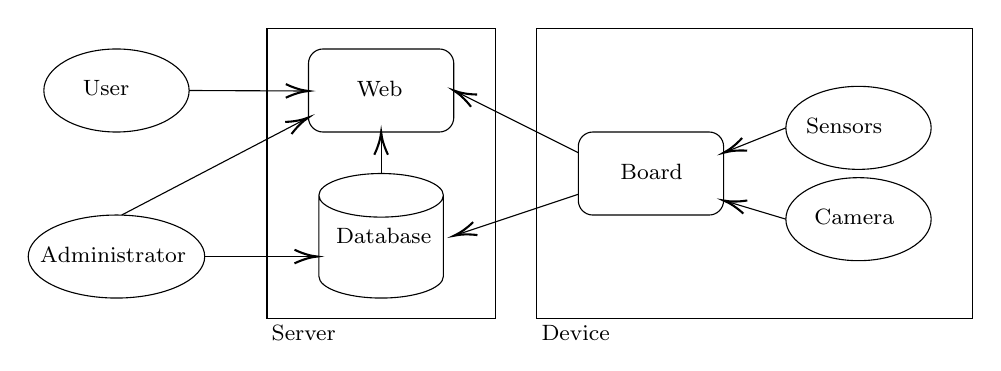
\begin{tikzpicture}[x=0.75pt,y=0.75pt,yscale=-1,xscale=1]

		\draw   (82.49,90) .. controls (82.49,78.95) and (98.16,70) .. (117.49,70) .. controls (136.82,70) and (152.49,78.95) .. (152.49,90) .. controls (152.49,101.05) and (136.82,110) .. (117.49,110) .. controls (98.16,110) and (82.49,101.05) .. (82.49,90) -- cycle ;

		\draw   (320,60) -- (530,60) -- (530,200) -- (320,200) -- cycle ;
		\draw   (440,108) .. controls (440,96.95) and (455.67,88) .. (475,88) .. controls (494.33,88) and (510,96.95) .. (510,108) .. controls (510,119.05) and (494.33,128) .. (475,128) .. controls (455.67,128) and (440,119.05) .. (440,108) -- cycle ;

		\draw   (275,140.5) -- (275,179.5) .. controls (275,185.3) and (261.57,190) .. (245,190) .. controls (228.43,190) and (215,185.3) .. (215,179.5) -- (215,140.5)(275,140.5) .. controls (275,146.3) and (261.57,151) .. (245,151) .. controls (228.43,151) and (215,146.3) .. (215,140.5) .. controls (215,134.7) and (228.43,130) .. (245,130) .. controls (261.57,130) and (275,134.7) .. (275,140.5) -- cycle ;

		\draw   (210,77) .. controls (210,73.13) and (213.13,70) .. (217,70) -- (273,70) .. controls (276.87,70) and (280,73.13) .. (280,77) -- (280,103) .. controls (280,106.87) and (276.87,110) .. (273,110) -- (217,110) .. controls (213.13,110) and (210,106.87) .. (210,103) -- cycle ;

		\draw   (340,117) .. controls (340,113.13) and (343.13,110) .. (347,110) -- (403,110) .. controls (406.87,110) and (410,113.13) .. (410,117) -- (410,143) .. controls (410,146.87) and (406.87,150) .. (403,150) -- (347,150) .. controls (343.13,150) and (340,146.87) .. (340,143) -- cycle ;

		\draw   (440,152) .. controls (440,140.95) and (455.67,132) .. (475,132) .. controls (494.33,132) and (510,140.95) .. (510,152) .. controls (510,163.05) and (494.33,172) .. (475,172) .. controls (455.67,172) and (440,163.05) .. (440,152) -- cycle ;

		\draw    (440,152) -- (411.92,143.57) ;
		\draw [shift={(410,143)}, rotate = 376.7] [color={rgb, 255:red, 0; green, 0; blue, 0 }  ][line width=0.75]    (10.93,-3.29) .. controls (6.95,-1.4) and (3.31,-0.3) .. (0,0) .. controls (3.31,0.3) and (6.95,1.4) .. (10.93,3.29)   ;
		\draw    (440,108) -- (411.86,119.26) ;
		\draw [shift={(410,120)}, rotate = 338.2] [color={rgb, 255:red, 0; green, 0; blue, 0 }  ][line width=0.75]    (10.93,-3.29) .. controls (6.95,-1.4) and (3.31,-0.3) .. (0,0) .. controls (3.31,0.3) and (6.95,1.4) .. (10.93,3.29)   ;
		\draw    (152.49,90) -- (208,90.24) ;
		\draw [shift={(210,90.25)}, rotate = 180.25] [color={rgb, 255:red, 0; green, 0; blue, 0 }  ][line width=0.75]    (10.93,-3.29) .. controls (6.95,-1.4) and (3.31,-0.3) .. (0,0) .. controls (3.31,0.3) and (6.95,1.4) .. (10.93,3.29)   ;
		\draw    (340,120) -- (281.79,90.89) ;
		\draw [shift={(280,90)}, rotate = 386.57] [color={rgb, 255:red, 0; green, 0; blue, 0 }  ][line width=0.75]    (10.93,-3.29) .. controls (6.95,-1.4) and (3.31,-0.3) .. (0,0) .. controls (3.31,0.3) and (6.95,1.4) .. (10.93,3.29)   ;
		\draw    (340,140) -- (281.9,159.37) ;
		\draw [shift={(280,160)}, rotate = 341.57] [color={rgb, 255:red, 0; green, 0; blue, 0 }  ][line width=0.75]    (10.93,-3.29) .. controls (6.95,-1.4) and (3.31,-0.3) .. (0,0) .. controls (3.31,0.3) and (6.95,1.4) .. (10.93,3.29)   ;
		\draw    (245,130) -- (245,112) ;
		\draw [shift={(245,110)}, rotate = 450] [color={rgb, 255:red, 0; green, 0; blue, 0 }  ][line width=0.75]    (10.93,-3.29) .. controls (6.95,-1.4) and (3.31,-0.3) .. (0,0) .. controls (3.31,0.3) and (6.95,1.4) .. (10.93,3.29)   ;
		\draw   (190,60) -- (300,60) -- (300,200) -- (190,200) -- cycle ;
		\draw   (74.97,170) .. controls (74.97,158.95) and (94.01,150) .. (117.49,150) .. controls (140.97,150) and (160,158.95) .. (160,170) .. controls (160,181.05) and (140.97,190) .. (117.49,190) .. controls (94.01,190) and (74.97,181.05) .. (74.97,170) -- cycle ;

		\draw    (160.2,170) -- (212.2,170) ;
		\draw [shift={(214.2,170)}, rotate = 180] [color={rgb, 255:red, 0; green, 0; blue, 0 }  ][line width=0.75]    (10.93,-3.29) .. controls (6.95,-1.4) and (3.31,-0.3) .. (0,0) .. controls (3.31,0.3) and (6.95,1.4) .. (10.93,3.29)   ;
		\draw    (120,150) -- (208.23,103.93) ;
		\draw [shift={(210,103)}, rotate = 512.4300000000001] [color={rgb, 255:red, 0; green, 0; blue, 0 }  ][line width=0.75]    (10.93,-3.29) .. controls (6.95,-1.4) and (3.31,-0.3) .. (0,0) .. controls (3.31,0.3) and (6.95,1.4) .. (10.93,3.29)   ;

		\draw (321,202) node [anchor=north west][inner sep=0.75pt]  [font=\footnotesize] [align=left] {Device};
		\draw (222,155) node [anchor=north west][inner sep=0.75pt] [font=\footnotesize] [align=left] {Database};
		\draw (232,84) node [anchor=north west][inner sep=0.75pt]  [font=\footnotesize] [align=left] {Web};
		\draw (191,202) node [anchor=north west][inner sep=0.75pt]  [font=\footnotesize] [align=left] {Server};
		\draw (100,84) node [anchor=north west][inner sep=0.75pt]  [font=\footnotesize] [align=left] {User};
		\draw (359,124) node [anchor=north west][inner sep=0.75pt]  [font=\footnotesize] [align=left] {Board};
		\draw (448.5,102) node [anchor=north west][inner sep=0.75pt]  [font=\footnotesize] [align=left] {Sensors};
		\draw (452.5,146) node [anchor=north west][inner sep=0.75pt]  [font=\footnotesize] [align=left] {Camera};
		\draw (79.49,164) node [anchor=north west][inner sep=0.75pt]  [font=\footnotesize] [align=left] {Administrator};

	\end{tikzpicture}}
\end{figure}

The system consists of:
\begin{itemize}
	\item \textbf{User:} Authorized personnel responsible for monitoring the images provided by the camera and monitoring the measurements transmitted by the sensors of the device.
	\item \textbf{Administrator:} Person in charge of the maintenance of the database and the website, as well as the proper reception of measurements and images. In the case of any incident, this person is responsible for resolving it.
	\item \textbf{Web:} Page where you can access the different devices, their measurements and video image.
	\item \textbf{Database:} Storage of user information, device information and the measurements they collect.
	\item \textbf{Server:} User-accessible place where the website and database are hosted.
	\item \textbf{Board:} Device where the various sensors and the camera are installed.
	\item \textbf{Sensors:} Devices sensitive to the different environmental factors to be measured in the DPC\@.
	\item \textbf{Camera:} A device that captures the image used for video surveillance.
	\item \textbf{Device:} Board, sensors and camera assembly.
\end{itemize}

\subsection{Use cases}\label{subsec:use-cases}
\begin{figure}[H]
	\ffigbox[\textwidth]
	{\caption{Use Cases Diagram}
		\label{fig:use_cases_diagram}}
	{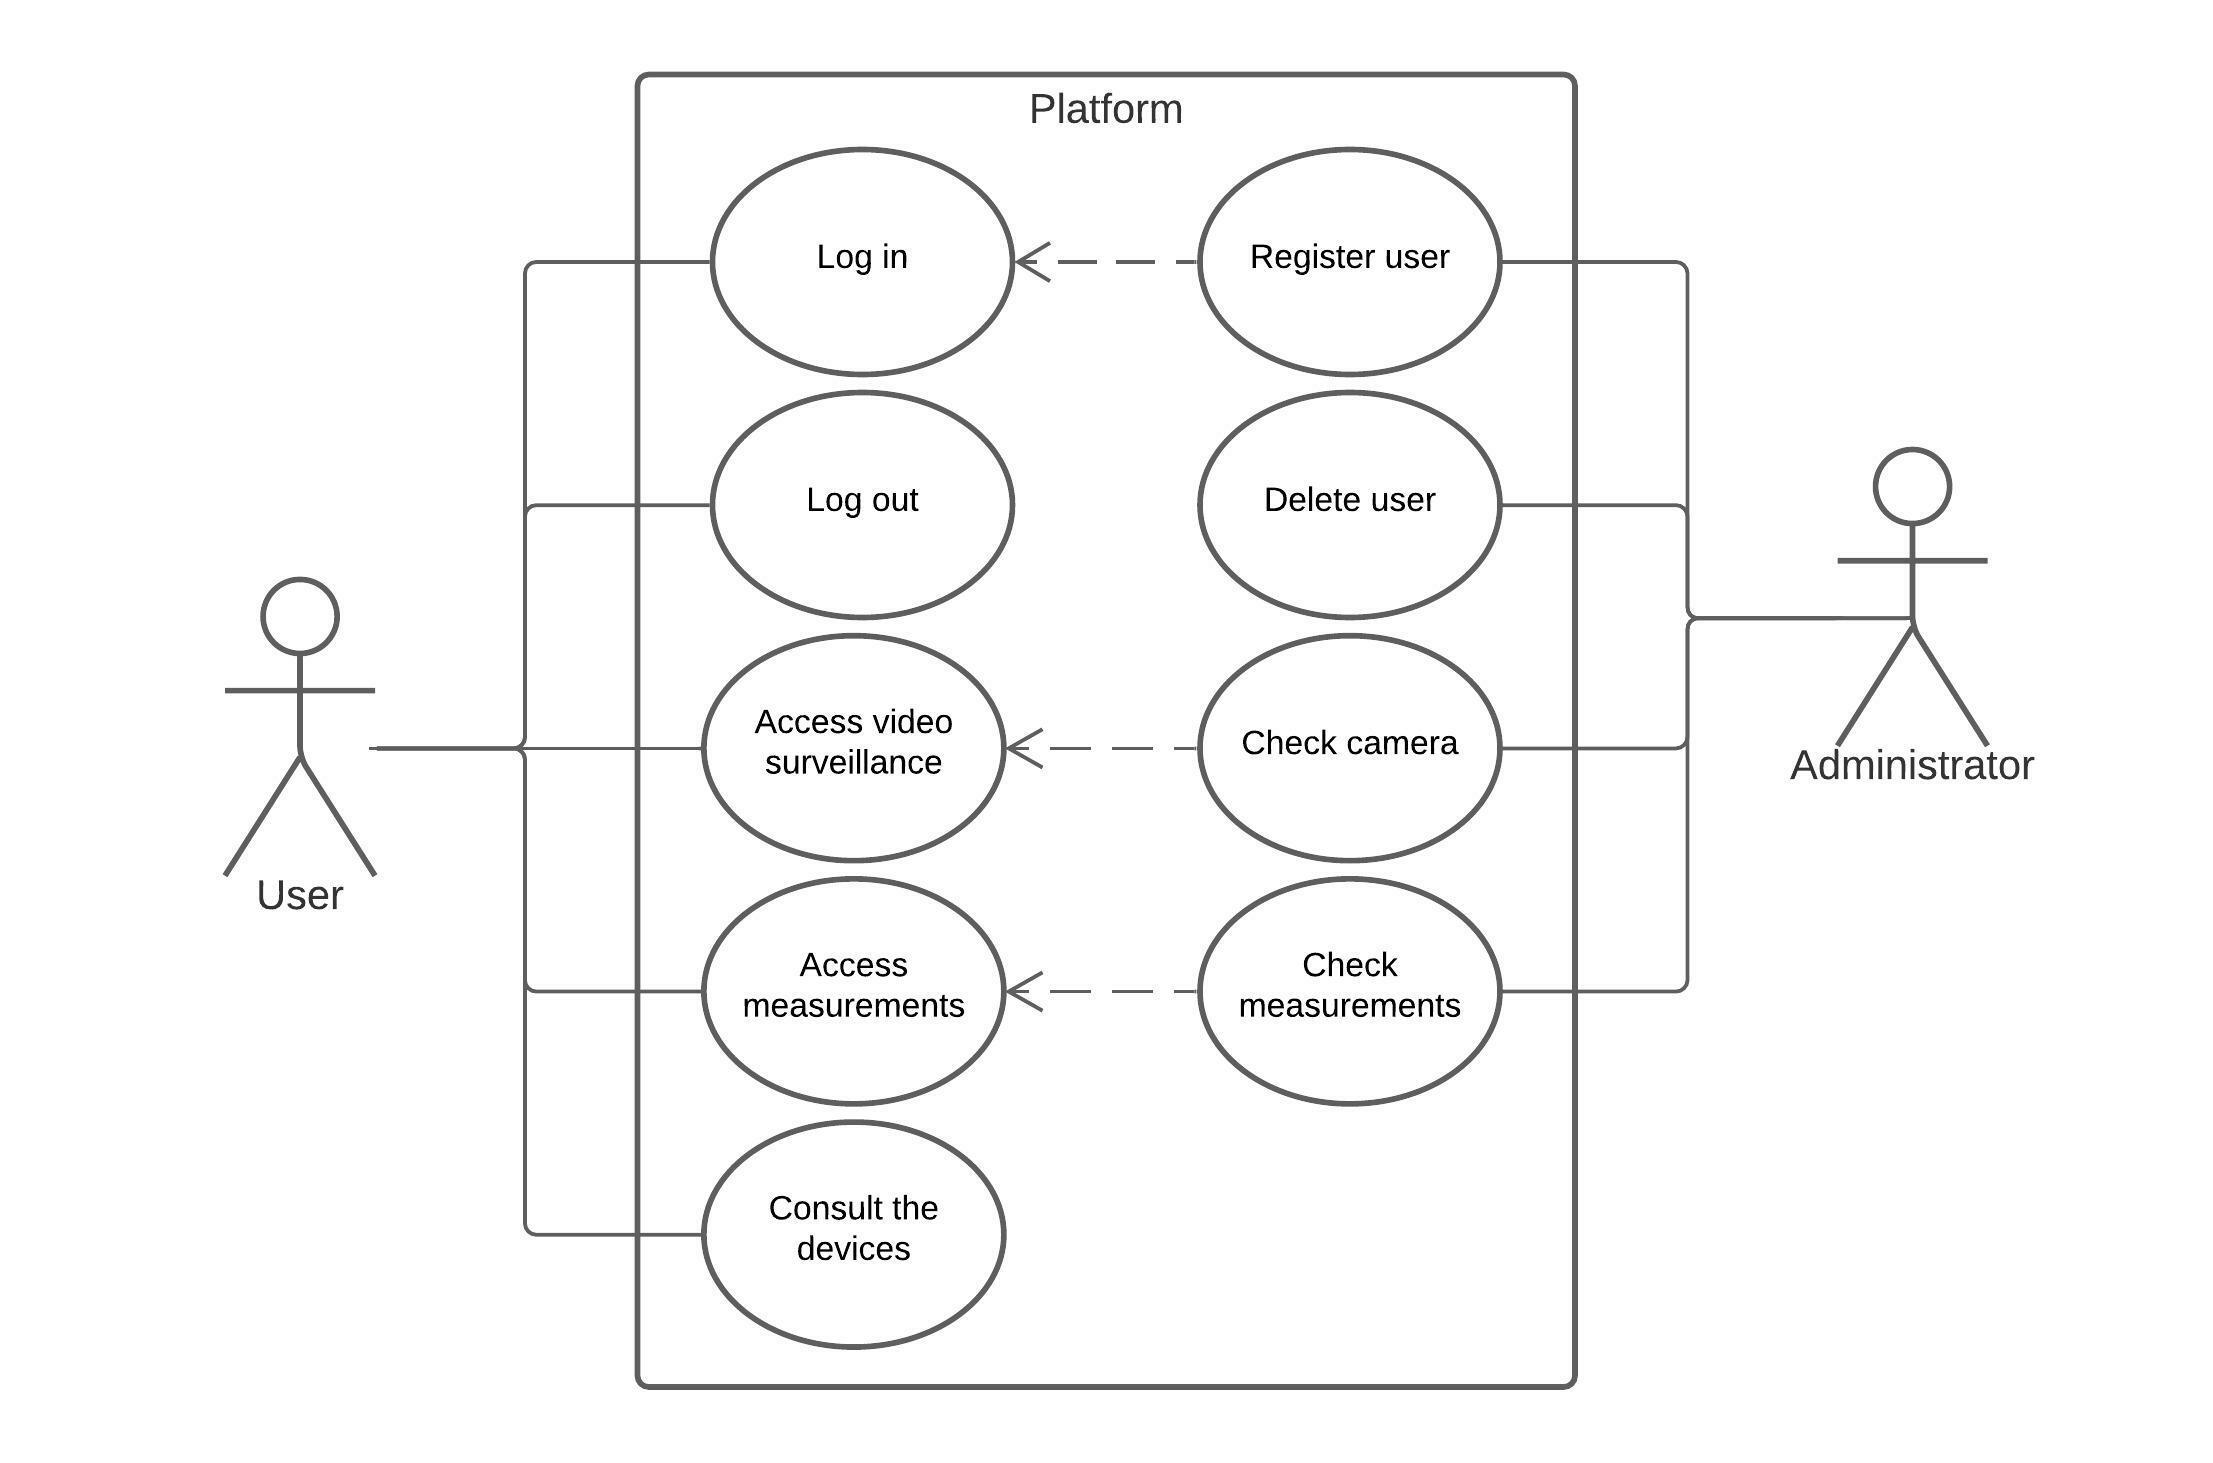
\includegraphics[scale=.7]{use_cases.jpeg}}
\end{figure}

\section{Design}\label{sec:design}
\subsection{Architecture}\label{subsec:architecture}
The system developed in this project follows the Model-View-Controller development pattern, which allows us to clearly separate the different parts of the system to be developed. This architecture is composed of the following parts:
\begin{itemize}
	\item \textbf{Model:} The part in charge of the logical representation of the information in the system, the mechanisms to access and store it. This will be the part related to the database.
	\item \textbf{View:} It is the visual representation of the system (web interface) that will be displayed to the user when using the application.
	\item \textbf{Controller:} It represents all the logic of the system, both the processing of measurements and the handling of requests to the server.
\end{itemize}

This separation into three parts makes it possible to develop and implement them in parallel so that everything is more modularized and can be modified or replaced without any problem.

\subsection{Components}\label{subsec:components}
This subsection discusses in more detail what the components that form the system will be, in the form of a component diagram, where the subsystems and components are:
\begin{itemize}
	\item \textbf{Device:} It represents all the devices that are connected to the system and that will take the measurements of the ambient and image of the interior of the room, that is why it is formed by the following components: Sensors, Camera and Board.
	\item \textbf{Database:} It represents the set of tables that constitute the data model, in which measurements, device data and user credentials shall be stored. Its components are User data, Measurement data and Device data.
	\item \textbf{Application:} This is the subsystem which the user interacts with, by using his credentials the user has access to see the connected devices, their measurements and the image taken by them. It is composed of: Login, List of devices, Measurements and Video surveillance.
\end{itemize}

\subsection{Data model}\label{subsec:data-model}
In this project, the database is one of the most important elements that compose the system, not only to allow authorized personnel access to the application, but also because it will store the history of the measurements taken in the room, which in the future will make it possible to analyse the state of the room.

The database will be hosted on the server, where the application will be able to access it more easily for viewing and consulting. It also facilitates the centralization of the measurements in a single place if there are multiple devices in a building and the user wishes to consult them from a single point.

\begin{itemize}
	\item \textbf{Table of users:} The credentials of the users using the application are stored in this table. These credentials are consulted when a user tries to log in and will be added by the system administrator in this table. It is important to note that the password is stored in hash format (encrypted) to prevent it from being read in case of intrusion.
	\item \textbf{Table of devices:} This table records the devices that have connected to the server, these devices are the ones that can be consulted from the application and are shown with the date of update along with their current status.
	\item \textbf{Table of measurements:} This is the most important table, where the measurements taken by all connected devices are stored. This data is displayed on the device's page within the application, along with its real-time image. The measurements that are stored are: temperature, humidity, PM$_{2.5}$, PM$_{10}$, CO and CO$_2$.
\end{itemize}

\subsection{User interface}\label{subsec:user-interface}
The user interface makes it possible for non-experts to use the system so that they can manipulate it and make use of it without the need to know how to develop a system of these characteristics.

The part of the system that has been provided with an interface is the part responsible for showing the measurements and video of the rooms. To accomplish this, a web page is used, which is designed in HTML and CSS, which allows access to all this information in a simple and visual way. The logic used to obtain the information and move through the screens is PHP\@.

The website is also responsive, so it is fully functional on both high-resolution devices and low-resolution devices.

The screens that compose the application are:
\begin{itemize}
	\item \textbf{Login:} This is the first screen the user will encounter when accessing the application. It is used to guarantee the security of the centre, so that unauthorized persons cannot access it.
	\item \textbf{Main:} Once the session has been successfully initiated, the user will be taken to this screen. Here you can see that it displays a greeting message, indicating the username.

	The key of this screen is the list of devices, where the device data is displayed in tabular form.
	\item \textbf{Device:} It shows the key information of this project, the image from the device camera and the measurements taken.
\end{itemize}

\section{Implementation}\label{sec:implementation}
The main method, \textit{start()}, starts the program and follows the next steps:
\begin{enumerate}
	\item Initialize the connection to the database and enter/update the status of the device, which changes it to Online status.
	\item Start camera transmission.
	\item Instantiate the temperature and humidity, suspended particles, CO and CO$_2$ sensors.
	\item A warm-up pause of 20 seconds for the sensors.
	\item In a loop, every 5 seconds, temperature and humidity, particulate matter, CO and CO$_2$ measurements are read and recorded in the database, along with the date and device id.
	\item If an interruption occurs, the GPIO port assignment is cleared, the particulate sensor is switched off and the last status update is sent indicating that the status is changed to Offline.
\end{enumerate}

\section{Project management}\label{sec:project-management}
\subsection{Planning}\label{subsec:planning}
The complete development of the product and its documentation took a total of 157 days. The following table shows the duration of the individual phases:
\begin{longtable}[c]{lcc|c|}
	\caption{Breakdown of planning by phases}
	\label{tab:phase_day_breakdown}\\
	\hline
	\rowcolor[HTML]{BFBFBF}
	\multicolumn{1}{|c|}{\cellcolor[HTML]{BFBFBF}{\color[HTML]{000000} \textbf{Activity}}} &
	\multicolumn{1}{c|}{\cellcolor[HTML]{BFBFBF}{\color[HTML]{000000} \textbf{\begin{tabular}[c]{@{}c@{}}Start\\ date\end{tabular}}}} &
	{\color[HTML]{000000} \textbf{\begin{tabular}[c]{@{}c@{}}End\\ date\end{tabular}}} &
	{\color[HTML]{000000} \textbf{\begin{tabular}[c]{@{}c@{}}Duration \\ (days)\end{tabular}}} \\ \hline
	\endfirsthead
	%
	\multicolumn{4}{c}%
	{{\bfseries Continuation of the Table \thetable\ on the previous page}} \\
	\hline
	\rowcolor[HTML]{BFBFBF}
	\multicolumn{1}{|c|}{\cellcolor[HTML]{BFBFBF}{\color[HTML]{000000} \textbf{Activity}}} &
	\multicolumn{1}{c|}{\cellcolor[HTML]{BFBFBF}{\color[HTML]{000000} \textbf{\begin{tabular}[c]{@{}c@{}}Start\\ date\end{tabular}}}} &
	{\color[HTML]{000000} \textbf{\begin{tabular}[c]{@{}c@{}}End\\ date\end{tabular}}} &
	{\color[HTML]{000000} \textbf{\begin{tabular}[c]{@{}c@{}}Duration \\ (days)\end{tabular}}} \\ \hline
	\endhead
	%
	\multicolumn{1}{|l|}{\textbf{Proposal}}                   & \multicolumn{1}{c|}{13-07-2021} & 20-07-2021     & 7   \\ \hline
	\multicolumn{1}{|l|}{\textbf{Previous documentation}}     & \multicolumn{1}{c|}{20-07-2021} & 08-08-2021     & 19  \\ \hline
	\multicolumn{1}{|l|}{\textbf{Project management}}         & \multicolumn{1}{c|}{08-08-2021} & 18-08-2021     & 10  \\ \hline
	\multicolumn{1}{|l|}{\textbf{Introduction}}               & \multicolumn{1}{c|}{18-08-2021} & 23-08-2021     & 5   \\ \hline
	\multicolumn{1}{|l|}{\textbf{State of the art}}           & \multicolumn{1}{c|}{23-08-2021} & 18-09-2021     & 26  \\ \hline
	\multicolumn{1}{|l|}{\textbf{Analysis}}                   & \multicolumn{1}{c|}{18-09-2021} & 01-10-2021     & 13  \\ \hline
	\multicolumn{1}{|l|}{\textbf{Design}}                     & \multicolumn{1}{c|}{01-10-2021} & 14-10-2021     & 13  \\ \hline
	\multicolumn{1}{|l|}{\textbf{Implementation}}             & \multicolumn{1}{c|}{14-10-2021} & 17-11-2021     & 34  \\ \hline
	\multicolumn{1}{|l|}{\textbf{Tests}}                      & \multicolumn{1}{c|}{17-11-2021} & 30-11-2021     & 13  \\ \hline
	\multicolumn{1}{|l|}{\textbf{Regulatory framework}}       & \multicolumn{1}{c|}{30-11-2021} & 03-12-2021     & 3   \\ \hline
	\multicolumn{1}{|l|}{\textbf{Socio-economic environment}} & \multicolumn{1}{c|}{03-12-2021} & 05-12-2021     & 2   \\ \hline
	\multicolumn{1}{|l|}{\textbf{Conclusions}}                & \multicolumn{1}{c|}{05-12-2021} & 09-12-2021     & 4   \\ \hline
	\multicolumn{1}{|l|}{\textbf{Summary/Abstract}}           & \multicolumn{1}{c|}{09-12-2021} & 15-12-2021     & 6   \\ \hline
	\multicolumn{1}{|l|}{\textbf{Acknowledgements}}           & \multicolumn{1}{c|}{15-12-2021} & 16-12-2021     & 1   \\ \hline
	\multicolumn{1}{|l|}{\textbf{Abbreviations}}              & \multicolumn{1}{c|}{16-12-2021} & 17-12-2021     & 1   \\ \hline
	                                                          &                                 & \textbf{Total} & 157 \\ \cline{4-4}
\end{longtable}

\subsection{Budget}\label{subsec:budget}
This subsection will gather and explain all the expenses that have been generated for the development of this project.

\begin{itemize}
	\item \textbf{Staff:} The cost associated with the salary to be paid to the staff in charge of this project. Although this work has been carried out by a single person, in a real team it would be made up of different professionals with different specialities such as: Project Manager, Analyst, Designer, Programmer and Test Manager.
	\item \textbf{Equipment and Components:} All the equipment used and the material used during the project have been considered, both the material that will form part of the developed product itself and the hardware needed to analyse, design, programme and test it.
	\item \textbf{Software:} The majority of the software used is free, and thanks to the student licences provided by UC3M, it has been possible to access some paid software.
	\item \textbf{Consumables:} Collects the cost of all material that is consumed and cannot be reused.
	\item \textbf{Travel and subsistence:} Costs associated with travel by public transport and one meal per week.
	\item \textbf{General expenses:} All expenses not covered above have been estimated at 15 \%, which include rent, electricity, telephone line, internet, cleaning, among others.
	\item \textbf{Industrial benefit:} A 6 \% profit will be received on the cost of the project.
\end{itemize}

All these budgets can be summarized as follows:
\begin{table}[H]
	\centering
	\caption{Budget summary}
	\label{tab:total_budget}
	\begin{tabular}{l|r|}
		\hline
		\rowcolor[HTML]{BFBFBF}
		\multicolumn{1}{|c|}{\cellcolor[HTML]{BFBFBF}\textbf{Budgets}} & \multicolumn{1}{c|}{\cellcolor[HTML]{BFBFBF}\textbf{Total Costs}} \\ \hline
		\multicolumn{1}{|l|}{Staff}                                    & €5,880.05                                                         \\ \hline
		\multicolumn{1}{|l|}{Equipment}                                & €304.47                                                           \\ \hline
		\multicolumn{1}{|l|}{Components}                               & €109.31                                                           \\ \hline
		\multicolumn{1}{|l|}{Software}                                 & €8.00                                                             \\ \hline
		\multicolumn{1}{|l|}{Consumables}                              & €34.88                                                            \\ \hline
		\multicolumn{1}{|l|}{Travel and subsistence}                   & €840.00                                                           \\ \hline
		\multicolumn{1}{|l|}{General expenses (15\%)}                  & €1.076,51                                                         \\ \hline
		\multicolumn{1}{|l|}{Industrial benefit (6\%)}                 & €495.19                                                           \\ \hline
		\multicolumn{1}{r|}{\textbf{Total (excluding VAT)}}            & €8,748.41                                                         \\ \cline{2-2}
	\end{tabular}
\end{table}

\noindent
The price of execution of the project reaches the amount of \MakeUppercase{eight thousand seven hundred and forty-eight and forty-one euros} (VAT not included).

\section{Conclusions}\label{sec:conclusions}
\subsection{Project conclusions}\label{subsec:project-conclusions}
Throughout this project, we have been able to see the process that is carried out when developing an environmental control and video surveillance system for a DPC. The objective has been to meet the needs of a client or person interested in this project.

The main and most important conclusion is that the project has been successfully developed, fulfilling all the objectives set out in the subsection of objectives.

Regarding the device, the necessary sensors have been installed for the proposed needs, while maintaining a low cost, as this was one of the key points to be achieved so that it could be widely implemented in all types of companies. Even with a low cost, all the modules installed work together and provide the necessary data to perform their task with suitable quality.

The choice of the Raspberry has been a complete success, as there is a lot of documentation on the internet and this has facilitated its programming and connection with the rest of the modules. On the other hand, some of the sensors that have been installed had no documentation and we had to research their internal specifications to be able to use them from the board.

Regarding the server, the desired database has been set up in which to store all the measurements of the devices, the status of the devices and the users. In addition, the web application is hosted on this server, which is accessible to anyone with the necessary permissions and has a simple and intuitive interface, as planned.

That said, it is worth mentioning that even if all the objectives had been met, the system could still perform significantly better if a higher budget were available, which was limited in this case. The use of these higher cost modules would only require minor modifications to the current project.

After all this, it is concluded that the system is fully functional, both the physical device part and the web application for monitoring the room in which it is installed.

\subsection{Personal conclusions}\label{subsec:personal-conclusions}
The development of this work has allowed me to get to know in more detail an aspect of computer science that has not been dealt with in depth during the degree, such as the development of physical devices. In addition, I have not only learnt about the development of this type of system at hardware level, but I have also been able to explore the field of IoT by connecting these devices to a central server.

Another of the technologies that I have been able to learn is PHP, one of the most widely used web programming languages nowadays. When I started this project, I basically knew HTML and JavaScript, so learning this new language has been more accessible to me, which I'm sure will be useful in my future job.

Not everything has been entirely new, I have also been able to put into practice much of the knowledge acquired throughout these years of study, such as programming, search techniques and use of information or software engineering, which have been essential to carry out this project.

I have been aware of the development of other skills such as time management, bibliography search, analysis and synthesis, decision-making and motivation.

With all this, I can say that it has been one of the projects that has brought me the most, not only academically, but also personally, due to all that it has involved.

\subsection{Future work}\label{subsec:future-work}
This project has been developed with the objective of being implemented in a data processing centre, but given its performance and price, it could be installed in other types of industries:
\begin{itemize}
	\item Animal protection enclosures, where animal monitoring and control is desired.
	\item Food handling rooms, where controlling the quality of the environment may mean avoiding possible intoxication.
	\item Certain hospital enclosures, where air quality determines possible infections.
\end{itemize}

In addition, the device is open to be connected to electrical, ventilation or fire extinguishing systems so that when it detects certain parameters it can act on them directly, without the need for someone to see it from the web and act manually.

On the other hand, the device is limited by the budget available for its development, so its properties could be improved by using, for example, a more powerful board, more precise sensors, more cameras per device and even other types of sensors.